\documentclass{article}

\usepackage{listings}
\usepackage{color}
\usepackage{graphicx}
\usepackage{float}

\title{Lab 1: Schematic Drawing Exercises}
\date{October 03, 2017}
\author{Matthew Friedman 861151348 \\ Souradeep Bhattacharya 861105938\\ EE128 Section: 021}

\begin{document}
	\maketitle
	
	\section*{Abstract}
	The objective of this lab was to familiarize ourselves with OrCad Capture CIS. To do so we built and modified 2 circuit schematics.
	\section*{Experiment System Specification}
	\subsection*{Part 1}
	Draft a timer using the 555 timing IC, resistors, and capacitors.
	\subsection*{Part 2}
	Setup an interrupt circuit for the MC9S12DJ128BCPV micro controller IC, and add LED’s to port B.
	
	\section*{Schematic Diagrams}
	\subsection*{Part 1}
	\begin{figure}[H]
		\centering
		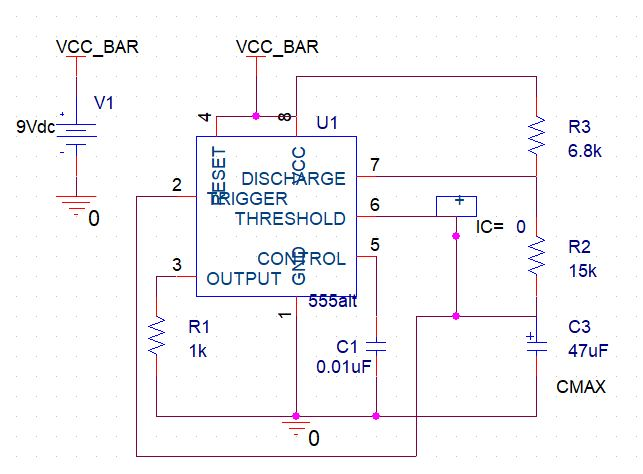
\includegraphics[width=1\textwidth]{part1}
	\end{figure}
	\subsection*{Part 2-A}
	\begin{figure}[H]
		\centering
		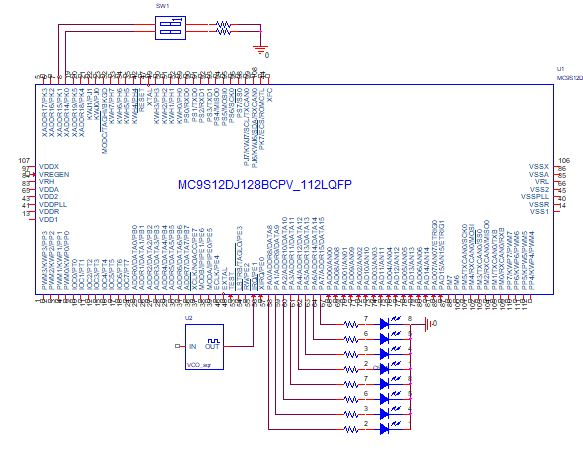
\includegraphics[width=1\textwidth]{part2}
	\end{figure}
	\subsection*{Part 2-B}
	\begin{figure}[H]
		\centering
		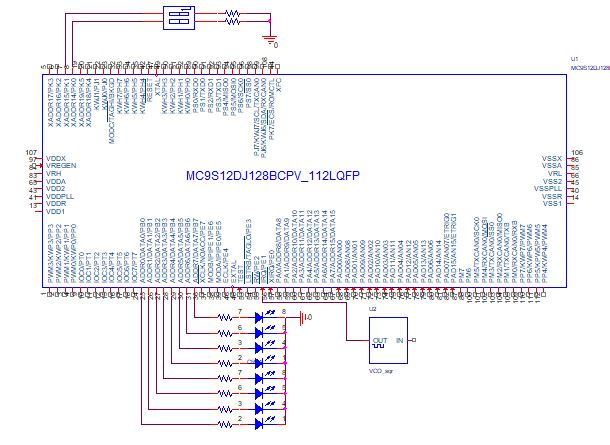
\includegraphics[width=1\textwidth]{part2b}
	\end{figure}
	
	\section*{Technical Problems}
	We had to install a secondary library that contained parts required for the lab. This was done by downloading the libraries from the iLearn site and adding them to the folder where the rest of the libraries were.
	\section*{Conclusion}
	In conclusion, we successfully refreshed our skills with OrCad Capture CIS by drafting and modifying 2 circuit schematics.
\end{document}